%% -----------------------------------------------------------
%% Estado del arte
%% -----------------------------------------------------------
\chapter{Estado del arte}
El presente análisis se desarrolló en el contexto de la evolución experimentada durante la última década por los modelos de IA en el estudio de la epilepsia mediante señales electroencefalográficas. Consiste en un mapeo conciso de diversos estudios comparativos \cite{wu_review_2025}, \cite{craik2019deep}, \cite{slamaComprehensiveReviewMachine2025}, y en la documentación de modelos que poseen un rendimiento destacado entre las métricas estándar requeridas para implementar modelos de IA en entornos clínicos.

\section{Enfoque integral y arquitecturas híbridas en la implementación de inteligencia artificial}
Para delimitar el análisis, se consideran como arquitecturas híbridas los modelos con una combinación de técnicas multiparadigma. Es decir, se contemplan las combinaciones de cualquier técnica de inteligencia artificial (desde lógica hasta profunda); entre estas se incluyen híbridos de aprendizaje profundo, híbridos de aprendizaje automático e híbridos entre aprendizaje automático y profundo. 

El auge de la implementación de modelos \textit{end-to-end}, principalmente de aprendizaje profundo, se atribuye a la omisión de la selección de características manuales, debido a que las capas internas de estos modelos aprenden de forma implícita las representaciones jerárquicas y abstractas de la señal. Dicha extracción favorece el rendimiento debido a su capacidad para modelar dependencias espacio-temporales. 

Sin embargo, su aplicación presenta dificultades ante la variabilidad entre sujetos, las diferencias entre los equipos de adquisición y la pérdida de trazabilidad de la información. El principal impedimento para su adopción clínica es su falta de interpretabilidad, debido a que estos modelos representan una caja negra que reduce la transparencia requerida para la toma de decisiones.

En contraste, se ha propuesto la combinación estratégica de metodologías y familias de algoritmos para solventar las deficiencias de ciertos componentes en el desempeño de los modelos. El Cuadro \ref{tab:matriz_modelos_actuales} presenta algunos de los paradigmas implementados y modelos representativos por sus métricas.

\begin{table}[h!]
    \centering
    \small
    \renewcommand{\arraystretch}{2.0}
    \setlength{\tabcolsep}{5pt}
    \captionsetup{width=0.95\linewidth}
    \caption{Matriz comparativa de los modelos actuales.}
    \resizebox{\textwidth}{!}{%
    \begin{tabular}{p{3cm} | p{3.5cm} p{3.5cm} p{3.5cm} p{2.5cm}}
    \hline
    \textbf{Modelo}     
    & \textbf{Técnica implementada}                
    & \textbf{Entradas o componentes}        
    & \textbf{Métricas reportadas}        
    & \textbf{Base de datos} \\ \hline
    
    \textbf{Swin-ViT}   
    & Aprendizaje profundo \textit{end-to-end}: \newline Transformadores de visión (\textit{ViT})
    & Análisis multimodal de imágenes 2D generadas a partir de EEG.
    & Exactitud: 96.34\,\% \newline Sensibilidad: 94.2\,\% \newline Especificidad: 97.8\,\% 
    & CHB-MIT Scalp EEG Dataset\\
    [1.8ex] 
    
    \textbf{LookAroundNet}            
    & Aprendizaje profundo \textit{end-to-end}: \newline Transformador de contexto temporal extendido
    & Series temporales multicanal de EEG continuo.          
    & Puntaje F1: 77.8\,\% \newline Sensibilidad: 69.2\,\% \newline Falsos positivos: 3.4/día 
    & Temple University Seizure Corpus (TUSZ)\\
    [1.8ex]
    
    \textbf{Log-Mel 2D-CNN}            
    & Aprendizaje profundo \textit{end-to-end}: \newline Convolución 2D sobre espectrogramas Log-Mel
    & Espectrogramas Log-Mel 2D adaptados a bandas de frecuencia de EEG.
    & Exactitud: 98.13\,\% \newline Sensibilidad: 95.33\,\% \newline Especificidad: 98.83\,\% \newline Puntaje F1: 95.32\,\%
    & Bonn University Dataset\\
    [1.8ex]
    
    \textbf{LHCAE \newline (3D-DCAE + BiLSTM)}            
    & Modelo híbrido: \newline Autocodificador convolucional 3D y Bi-LSTM
    & Registros EEG multicanal en ventanas fijas de 4~s.
    & Exactitud: 99.08 $\pm$ 0.54\,\% \newline Sensibilidad: 99.21 $\pm$ 0.50\,\% \newline Especificidad: 99.11 $\pm$ 0.57\,\% \newline Puntaje F1: 99.16 $\pm$ 0.50\,\%
    & CHB-MIT Scalp EEG Database\\
    [1.8ex]
    
    \textbf{LG-TriCapsNet}            
    & Arquitectura híbrida de grafos y cápsulas: \newline Grafos (NNG) y redes de cápsulas
    & Grafos de conectividad espacial y vectores de cápsulas.
    & Exactitud: 98.34\,\% \newline Sensibilidad: 98.3\,\% \newline Especificidad: 98.4\,\% \newline Puntaje F1: 98.32\,\%
    & Conjuntos públicos multienfermedad\\
    [1.8ex]
    
    \textbf{IG-Based DNN}            
    & Aprendizaje híbrido: \newline Selección por ganancia de información (IG) + DNN
    & Atributos fisiológicos explícitos de la señal.         
    & Exactitud: 99.0\,\% \newline Puntaje F1: 99.0\,\% 
    & Bonn University Dataset\\ \hline
    \end{tabular}
    }
    
    \vspace{2mm}
    \small \textit{Nota: Resumen de desempeños reportados en la literatura para arquitecturas de referencia. Elaboración propia.}
    \label{tab:matriz_modelos_actuales}  
\end{table}

Al margen de las especificaciones arquitectónicas individuales, la dicotomía evidente en las arquitecturas analizadas en el Cuadro \ref{tab:matriz_modelos_actuales} se puede abstraer al contraste entre la extracción automatizada de representaciones de la señal y la ingeniería de características. La coexistencia de estos paradigmas en su implementación se rige por sus fortalezas y limitaciones.

\subsection{Descomposición e ingeniería de características}
Este enfoque se fundamenta en el conocimiento experto de la neurofisiología y el procesamiento de señales digitales. La descomposición y extracción de atributos se realiza mediante métricas estadísticas en el dominio temporal, frecuencial y tiempo-frecuencia. Debido a la variedad de atributos, se incorporan métodos de selección y reducción como los filtros de ganancia de información (IG), análisis de componentes principales (PCA), entre otros.

Sus mayores fortalezas radican en su alta interpretabilidad clínica y matemática, la eficiencia computacional, variabilidad en el borde y robustez con escasez de datos. En contraste, se ve limitado por la incapacidad para capturar interacciones espacio-temporales y el sesgo humano y carga de ajuste manual.

\subsection{Aprendizaje de \textit{end-to-end}}
Paradigma que prescinde de la ingeniería de características. En el caso analizado, la entrada del sistema es la señal EEG cruda o representaciones de formato visual global y delega a las capas profundas de la red la tarea de aprender automáticamente la jerarquía de abstracción.

Entre sus principales ventajas están la extracción automática y libre de sesgo, modelado de dinámicas no lineales y multicanal y el potencial de rendimiento teórico. Sin embargo, está limitado por el efecto de caja negra debido a la opacidad de los millones de parámetros de la red, costo computacional extremo y altamente propensos al sobreajuste.

\subsection{Enfoque híbrido}
A partir de la utilidad de cada modelo, la literatura ha convergido hacia \textit{sistemas híbridos} para cubrir las exigencias clínicas. Fundamentado en su propósito, es posible identificar cinco familias aplicadas de modelos híbridos.

\subsubsection{Híbrido espacio-temporal}
Se enfocan en el análisis de tanto las secuencias temporales como la extracción de patrones espaciales y espectrales locales. Algunos modelos ejemplares son LHCAE que consiste en un autocodificador convolucional 3D y un Bi-LSTM \cite{srinivasan2023detection}, y un CNN+LSTM \cite{dasEnhancedEEGSignal2025}. 

\subsubsection{Híbrido topológico y de conectividad}
Capturan la estructura no euclidiana del cerebro y la conectividad funcional y/o espacial de los electrodos. Abordan las dificultades en el rendimiento debido a la heterogeneidad interpacientes. Entre estos están LG-TriCapsNet que consiste en la fusión de grafos de vecinos más cercanos y redes de cápsulas \cite{jain2025lg} y FPMBGCN que consiste en redes de grafos multirrama \cite{zhangFPMBGCNFeaturePyramidbased2026}

\subsubsection{Híbridos de reducción y dominio explicable}
Priorizan reducir la incertidumbre de las cajas negras, la exigencia computacional y el sobreajuste de los modelos profundos. Ciertos modelos representativos son IG-Based Hybrid + DNN \cite{ikizlerEpilepticSeizureDetection2026}, el cual consiste en la aplicación de características de tiempo, frecuencia y wavelets filtrados por IG introducidos a una red DNN ligera; y Compressive Sensing + XGBoost \cite{djemal2025fast}, que comprime la señal hasta en un 70\% para realizar la clasificación mediante XGBoost en sistemas embebidos.

\subsubsection{Híbridos de incertidumbre metaheurística}
Resuelven la fragilidad de las redes tradicionales ante la alta no linealidad, inestabilidad y datos ambiguos imprecisos, moldeando la incertidumbre inherente de las señales cerebrales para optimizar los hiperparámetros de la red. Entre los modelos ejemplares está DT-FIS + WCA-AE + SFOA \cite{lak2026hybrid}, el cual integra un sistema de inferencia difusa basado en árboles de decisión a autocodificadores optimizados. 

\subsubsection{Híbridos de fusión de representaciones}
Evitan la pérdida de información en el procesamiento de las señales EEG en una sola dimensión, integran de forma coordinada las firmas temporales, de escala y de frecuencia de la crisis epiléptica. Un modelo referente es el Mix-ViT o Swin-ViT \cite{abualhassanEpilepticSeizureDetection2026}, que combina y fusiona mediante capas de atención aprendida, la señal cruda, espectrogramas Log-Mel y escalogramas CWT.

\section{Detección y remoción de artefactos}
En la literatura de detección y predicción de convulsiones mediante señales EEG, una de las causas primarias de las altas tasas de falsos positivos se atribuye a la confusión con artefactos. Su similitud morfológica y espectral genera que se identifiquen las variaciones bruscas de voltaje, ondas rítmicas de alta frecuencia o picos similares a las espigas epileptiformes como eventos epileptiformes \cite{afsariArtificialIntelligenceEpileptic2026}.

Para abordar este factor, se han aplicado cinco estrategias que se enfocan en aumentar el conocimiento desde diversas perspectivas.

\subsection{Módulos dedicados y pre-filtros}
Se implementan módulos livianos para el análisis continuo de la señal y asignación de la calidad del registro \cite{afsariArtificialIntelligenceEpileptic2026}, se introducen métodos de eliminación de artefactos con módulos específicos como filtros previos \cite{slamaComprehensiveReviewMachine2025}; y la implementación de bloques de pesaje adaptativo de canales, los cuales suprimen de forma automática el ruido o información no relevante en los canales \cite{zhangFPMBGCNFeaturePyramidbased2026}.

\subsection{Descomposición estadística y separación ciega de fuentes}
La técnica tradicional para descomponer la señal multicanal e identificar componentes asociados a los artefactos biológicos, técnicos y ambientales es la identificación de componentes independientes (ICA) \cite{craik2019deep, dasEnhancedEEGSignal2025, djemal2025fast, slamaComprehensiveReviewMachine2025, wu_review_2025}. Otro método utilizado para analizar las etapas previas y las amplitudes anómalas es mediante la transformada Wavelet discreta (DWT), sin distorsionar los picos epilépticos \cite{djemal2025fast}.

\subsection{Contexto temporal extendido}
Un método no invasivo consiste en el aumento de las ventanas de análisis de la señal \cite{sverrisson2026lookaroundnet}, aplicado en el modelo \textit{LookAroundNet}, el cual aporta contexto al transformador para una elevación brusca de la amplitud y aislamiento de la perturbación, reduciendo los falsos positivos.

\subsection{Fusión multimodal}
Integración de las señales de electrocardiogramas (ECG), electromiogramas (EMG) y/o video electroencefalogramas (VEEG) para corroborar si la alteración se debe a un artefacto \cite{afsariArtificialIntelligenceEpileptic2026}.

\subsection{Postprocesamiento y antirrebotes}
Para evitar que los picos aislados se identifiquen como actividad epileptiforme se aplican esquemas de decisión, filtros de media móvil y periodos refractarios \cite{wu_review_2025, wang2025eeg}.

\section{Clasificación de eventos y convulsiones}
Según las aplicaciones más recientes de modelos de aprendizaje profundo para la clasificación de crisis epilépticas como la convolución 1D/TCN \cite{wang2025eeg}, convolución 2D sobre representaciones tiempo-frecuencia \cite{sahatchindaDiagnosisEpilepticSeizures2025}. Reportan que se ha alcanzado un equilibrio entre la eficiencia computacional y la riqueza de representación. La convolución de una dimensión y la red convolucional temporal (TCN) se destaca por su eficiencia, identifican patrones temporales y dependencias secuenciales con bajos recursos. Y el análisis convolucional de dos dimensiones analiza una representación de tiempo-frecuencia, lo cual permite la captura de características espectrales complejas y un rendimiento eficiente ante el ruido.  

A pesar de que las representaciones de varias dimensiones permitan el análisis y captura de características espectrales y topográficas, todas estas arquitecturas están limitadas ante la generalización interpaciente debido a su ajuste a los patrones cerebrales de entrenamiento. Por lo tanto, la literatura demuestra que el rendimiento óptimo no recae en el paradigma puro, sino en arquitecturas híbridas como extractores de características latentes potentes y clasificadores tradicionales que proporcionan una decisión clínica auditable.

\section{Relevancia de la inteligencia artificial explicable (XAI)}
Partiendo de la premisa de que las arquitecturas profundas propuestas en el estado del arte operan como modelos de cajas negras, su implementación clínica enfrenta varios retos. Los neurólogos y personal médico requieren de plausibilidad fisiológica \cite{ahmadAdvancedMultimodalLearning2026} y validación regulatoria, por lo que la aplicación de métodos de explicabilidad es fundamental para auditar las propuestas, validar la toma de decisiones y cerrar la brecha de comunicación entre el modelo y el especialista, garantizando la confianza clínica.

En sistemas híbridos como los analizados previamente, es indispensable la aplicación de técnicas de explicabilidad para los segmentos de aprendizaje profundo. A nivel de señales EEG se reporta el uso de modelos de atribución de características (SHAP y LIME) \cite{ahmadAdvancedMultimodalLearning2026}, visualización de activación (Grad-CAM, mapas de saliencia y LRP) \cite{ahmadAdvancedMultimodalLearning2026}, selección explícita de atributos (IG) \cite{ahmadAdvancedMultimodalLearning2026} y métodos de causalidad.

\section{Estandarización de la evaluación de los modelos}
Las revisiones sistemáticas \cite{wu_review_2025, slamaComprehensiveReviewMachine2025, afsariArtificialIntelligenceEpileptic2026, craik2019deep} abordan el problema de variabilidad de las métricas de rendimiento y la falta de estandarización. Entre los sesgos sobresalen el cambio entre la evaluación de laboratorio y la aplicación clínica, la disparidad en ventanas temporales y la discrepancia entre las métricas tradicionales y clínicas. 

En respuesta a estas deficiencias en la comparación de los modelos, SzCORE \cite{danSzCOREBenchmarkReport2025} se presenta como un recurso para la estandarización, publicado bajo revisión de la comunidad científica en la revista \textit{Epilepsia} y marco implementado en la conferencia internacional \textit{Artificial Intelligence in Epilepsy and Neurological Disorders} de 2025. Los principales estándares que presenta son
\begin{itemize}
    \item Unificación de la metodología de validación bajo un mismo marco.
    \item Establece directrices integrales para la estructuración de las bases de datos.
    \item Define los formatos de organización de datos a los formatos propuestos BIDS-EEG y HED-SCORE.
    \item Propone un sistema de puntuación basado en eventos, permitiendo contabilizar uniformemente los verdaderos positivos, falsos positivos y falsos negativos.
\end{itemize}

Principalmente, su marco permite la restricción de métricas de rendimiento basándose en los eventos clínicos. Por ejemplo, la ecuación (\ref{ec:sensibilidad}) define la sensibilidad como la proporción de eventos reales que el algoritmo logra detectar con éxito.

\begin{equation}
    \text{Sensibilidad} = \frac{\text{TP}}{\text{TP} + \text{FN}}
    \label{ec:sensibilidad}
\end{equation}

Asimismo, la confiabilidad de las alertas generadas se evalúa mediante la precisión (ecuación \ref{ec:precision}), la cual representa la proporción de alertas generadas que realmente corresponden al evento.
\begin{equation}
    \text{Precisión} = \frac{\text{TP}}{\text{TP}+\text{FP}}
    \label{ec:precision}
\end{equation}

Para obtener un balance entre la sensibilidad y precisión del modelo se evalúa la puntuación F1 (ecuación \ref{ec:f1}), que constituye la media armónica entre ambos parámetros.
\begin{equation}
    \text{F1} = \frac{2\times \text{TP}}{2\times \text{TP}+\text{FN}+\text{FP}}
    \label{ec:f1}
\end{equation}

Para asegurar su desempeño a nivel clínico, se audita la cantidad de detecciones erróneas normalizadas en un periodo de monitoreo, la ecuación \ref{ec:fppd} define un intervalo continuo de 24 horas.
\begin{equation}
    \text{FP/24h} = \frac{FP}{\text{Horas totales de monitoreo}}\times 24
    \label{ec:fppd}
\end{equation}

%% -----------------------------------------------------------
%% Metodología y arquitectura
%% -----------------------------------------------------------
\chapter{Metodología y arquitectura propuesta}
A partir de los aportes del estado del arte en el diagnóstico de la epilepsia, se identificaron los retos derivados de analizar datos de alta dimensionalidad y de la exigencia de explicabilidad clínica. Para abordar estas limitaciones, el análisis se estructuró mediante sistemas modulares que permiten la centralización del conocimiento de distintos segmentos de estudio, utilizando los registros de la base de datos de \textit{Temple University Hospital} (TUH) \cite{obeid2016temple}. 

\begin{figure}[h] 
    \centering\captionsetup{width=0.8\linewidth}
    \caption{Marco de trabajo modular}
    \definecolor{blue_gray}{HTML}{6A8BA2}
\definecolor{white}{HTML}{FFFFFF}
\definecolor{light_blue}{HTML}{0F469F}
\definecolor{dark_blue}{HTML}{153657}
\definecolor{gray}{HTML}{474747}

\begin{tikzpicture}[
    node distance=1cm,
    bloque/.style={
        rectangle,
        draw=blue!60!black,
        fill=blue!8,
        rounded corners,
        minimum width=3.5cm,
        minimum height=1cm,
        align=center
    },
    flecha/.style={
        -{Stealth},
        thick
    }
]

\node[bloque, 
    draw = dark_blue,
    fill = blue_gray,
    text = white, 
] (entrada) {Señales EEG};

\node[bloque, 
    below=of entrada,
    draw = dark_blue,
    fill = blue_gray,
    text = white
] (processing) {Preprocesamiento generalizado};

\node[bloque,
    below left=1cm and 2.5cm of processing.south,
    draw=dark_blue,
    fill=light_blue,
    text=white
] (modulo1) {Detección de artefactos};

\node[bloque,
    below = of processing,
    draw=dark_blue,
    fill=light_blue,
    text=white
] (modulo2) {Clasificación de eventos};

\node[bloque,
    below right=1cm and 2.5cm of processing.south,
    draw=dark_blue,
    fill=light_blue,
    text=white
] (modulo3) {Clasificación de convulsiones};

\node[bloque,
    below = of modulo2,
    draw=dark_blue,
    fill=white,
    text=gray
] (cierre) {Módulo de apoyo a la decisión};

% Ramificación
\draw[flecha] (entrada.south) -- (processing.north);
% División y lineas centrales
\coordinate (division1) at ([yshift=-0.5cm]processing.south);
\draw[thick] (processing.south) -- (division1); 
% Arrows
\draw[flecha] (division1) -| (modulo1.north);
\draw[flecha] (division1) -| (modulo2.north);
\draw[flecha] (division1) -| (modulo3.north);

% División y lineas centrales
\coordinate (division2) at
    ([yshift=-0.5cm]modulo2.south);
\draw[thick] (modulo1.south) |- (division2);
\draw[thick] (modulo2.south) -- (division2);
\draw[thick] (modulo3.south) |- (division2);
% Arrow
\draw[flecha] (division2) -- (cierre.north);

\end{tikzpicture}

    \note{La imagen muestra el diagrama de flujo de la distribución modular propuesta como marco metodológico. Elaboración propia.}
    \label{fig:framework}   
\end{figure}

La metodología se delimitó a partir de los modelos detallados en el estado del arte, priorizando modelos preentrenados para optimizar la transferencia de aprendizaje y clasificadores tradicionales. En esencia, para cada actividad del sistema inteligente se contrastó un modelo \textit{end-to-end} con un esquema de extracción de características mediante modelos profundos y clasificación tradicional. De acuerdo con la estructura de la base de datos TUH, el problema se dividió en tres ejes: \textit{artefactos}, \textit{eventos y convulsiones}, y \textit{apoyo al diagnóstico de la epilepsia}, como se visualiza en la Figura \ref{fig:framework}

\section{Evaluación preliminar}
La fase exploratoria consistió en la validación conceptual del trabajo mediante la aplicación de técnicas de Inteligencia Artificial Explicable (XAI). El propósito de esta sección es auditar el comportamiento de algunos modelos implementados en la Universidad del Valle de Guatemala (UVG) y de las arquitecturas preentrenadas tomadas de referencia para cada módulo. 

\subsection{Aplicación de métodos de explicabilidad}
\subsubsection{Transformer temporal}
Como parte de la linea de investigación en UVG, la primera acción fue identificar los modelos entrenados disponibles para la evaluación mediante métodos de interpretabilidad (XAI). 
Según los datos reportados por Sanchez \cite{Sanchez_2025} y la disponibilidad del modelo \textit{Temporal transformer}, se utilizaron métodos agnósticos al modelo para analizar solamente la interacción de las entradas y salidas del modelo, como caja negra.
Aplicando principalmente el análisis de oclusión \autoref{ssub:xai_oclussion}

% Convenci\'on: valor = logit(original) - logit(ocultado). Positivo = empujaba hacia crisis.
% Ablation_summary.csv, summary_features_*.csv, direction_features_*.csv y features.parquet.
\begin{table}[htbp]
\centering
\small
\label{tab:muestra}
\begin{tabular}{lrrrr}
\toprule
Grupo & Ventanas & Pacientes & Logit (mediana) & $P$(crisis) (mediana) \\
\midrule
VP & 30 & 4 & 1.58 & 0.8299 \\
FP & 13 & 2 & 0.83 & 0.6973 \\
VN & 285 & 19 & $-$8.23 & 0.0003 \\
FN & 251 & 20 & $-$8.30 & 0.0002 \\
\bottomrule
\end{tabular}
\end{table}


\begin{table}[h!]
    \centering
    \small
    \renewcommand{\arraystretch}{2.0}
    \setlength{\tabcolsep}{5pt}
    \captionsetup{width=0.95\linewidth}
    \caption{Muestra analizada por grupo de la matriz de confusión (umbral 0.5). Las ventanas provienen de un muestreo estratificado por paciente, por lo que no son los conteos totales del conjunto de prueba.}
    \resizebox{\textwidth}{!}{%
    \begin{tabular}{c|ccccc}
    \hline
    Grupo & Ventanas & Pacientes & Logit (mediana) & $P$(crisis) (mediana) \\
    \hline
    VP & 30 & 4 & 1.58 & 0.8299 \\
    FP & 13 & 2 & 0.83 & 0.6973 \\
    VN & 285 & 19 & $-$8.23 & 0.0003 \\
    FN & 251 & 20 & $-$8.30 & 0.0002 \\
    \vspace{2mm}
    \small \textit{Nota: Resumen de desempeños reportados en la literatura para arquitecturas de referencia. Elaboración propia.}
    \label{tab:muestras}  
\end{table}

\begin{table}[htbp]
\centering
\small
\caption{Ablación por rama: caída del logit, $\mathrm{logit}(x)-\mathrm{logit}(x_{\mathrm{ablado}})$. Mediana por paciente y luego entre pacientes. Positivo: la rama empujaba hacia crisis; negativo: hacia no crisis.}
\label{tab:ramas}
\begin{tabular}{lrrrr}
\toprule
Perturbación & VP & FP & VN & FN \\
\midrule
Ablar señal (22 canales) & $-$0.19 & 0.00 & 0.00 & $-$0.01 \\
Ablar features (baseline 0) & 4.18 & 3.48 & $-$5.01 & $-$5.46 \\
Ablar features (media interictal) & 6.30 & 5.21 & $-$1.13 & $-$1.05 \\
Ablar ambas ramas & 4.19 & 3.49 & $-$5.00 & $-$5.45 \\
\bottomrule
\end{tabular}
\end{table}

\begin{table}[htbp]
\centering
\small
\caption{Ablación por familia de features (caída del logit), con baseline 0 y con la media interictal de cada paciente.}
\label{tab:familias}
\begin{tabular}{lrrrrrrrr}
\toprule
& \multicolumn{4}{c}{Baseline 0} & \multicolumn{4}{c}{Media interictal} \\
\cmidrule(lr){2-5}\cmidrule(lr){6-9}
Familia & VP & FP & VN & FN & VP & FP & VN & FN \\
\midrule
Amplitud & 1.88 & $-$0.55 & $-$0.66 & $-$2.41 & 0.07 & $-$0.58 & $-$0.21 & $-$0.89 \\
Energía & 2.69 & 8.31 & $-$0.55 & $-$0.74 & 2.00 & 6.44 & $-$0.09 & $-$0.26 \\
Potencia relativa & 9.54 & 2.78 & $-$1.69 & $-$0.28 & 8.81 & 1.98 & $-$0.42 & 0.49 \\
Ratios & 0.15 & $-$1.90 & $-$0.17 & $-$0.38 & 0.15 & $-$1.31 & 0.01 & $-$0.24 \\
Forma espectral & $-$0.76 & 3.55 & $-$0.85 & $-$0.44 & 0.07 & 2.72 & $-$0.18 & 0.18 \\
\bottomrule
\end{tabular}
\end{table}


\subsubsection{Large EEG-U-Transformer}

\section{Fundamento del enfoque híbrido}
El énfasis y sesgo en la implementación de arquitecturas de aprendizaje profundo en los últimos años, ha permitido la identificación de sus limitaciones. 
Las cuales se concentran en la mencionada baja interpretabilidad clínica, el sobreajuste y escasez de datos etiquetados y su baja generalización cruzada entre pacientes. 
Dicho sobreajuste genera un sesgo en las características aprendidas por el modelo, generalmente asociado a las características demográficas de los pacientes incluidos en la base de datos de entrenamiento. 

El enfoque híbrido considerado en el presente trabajo consiste en la implementación de los modelos de aprendizaje profundo como extractores temporales y espaciales, lo que implica una sección de seleción de características aprendidas de la naturaleza dinámica y multidimensional de las señales EEG. Arquitecturas como las redes convolucionales (CNN), convoluciones en profundidad y redes de grafos aprenden correlaciones, conectividad funcional y propagación de paroxismos a través de electrodos \cite{Lawhern2018EEGNet}.
Los algoritmos tradicionales tratan las ventanas de tiempo como bloques estáticos, perdiendo la continuidad secuencial y el contexto histórico de la señal.
Las redes recurrentes (BI-LSTM y GRU), redes convolucionales temporales (TCN) y \textit{Trasnformers} capturan la dinámica temporal, patrones rítmicos sostenidos y dependencias de largo alcance \cite{sahatchindaDiagnosisEpilepticSeizures2025}.
Un modelo de aplicación de extracción con modelos profundos y clasificación clásica, aborda la aplicación de autocodificadores con XGBoost y máquinas de vectores de soporte difusas, el cual reporta alcanzar una puntuación F1 del 99.28\% en la detección de crisis.
Bajo la observación que este modelo fue entrenado y evaluado con una base de datos diferente a la implementada en este estudio (\textit{CHB-MIT}).

\section{Arquitectura del módulo de artefactos}
La gestión de artefactos fisiológicos y extrafisiológicos en las señales EEG, se ha aplicado en tres enfoques estratégicos: reducción de falsos positivos y falsas alarmas clínicas, mejora de la relación señal-ruido y la preservación de datos sin descarte masivo.
Es decir, pasar del descarte completo de la información debido a la identificación de algún artefacto contra la ponderación y/o capacidad de limpieza de la señal.

Uno de los métodos con mayor consolidación, es el método de análsis de componentes independientes (ICA). Como se aborda en \ref{Marcoteorico_ICA} permite la separación de fuentes de interferencia mediante una selección estadística que se fundamenta en una maximización de la no-gaussianidad, en contraste con métodos de corte de umbral que es propenso a eliminar información relevante de la señal.
Los modelos profundos con base tradicional más extendida en la detección y eliminación de artefactos en EEG son las CNN (CNN-LSTM y GAN-\textit{Transformers}) y los autocodificadores (AE). Dichos modelos aprenden de patrones jerárquicos y representaciones complejas de la señal, comprimen la alta dimensionalidad a un espacio latente compacto, preservando los atributos neurofisiológicos y descartando información redundante \cite{mouazenTransparentEEGAnalysis2025}. 
Como referencia para el análisis de detección de este tipo de redes es la aplicación de tres modelos CNN, cada uno especializado para una categoría \cite{Nyanney2026ArtifactsCNN}.
Dicho trabajo, plantea la implementación de tres CNN binarios independientes y especializados, bajo el enfoque de presentar un modelo ligero y alta especificidad clínica (del 96 al 98.2 \%).

Considerando la preservación de la morfología que permite ICA, la metodología propuesta consiste en el contraste de dos enfoques: el análisis de la descomposición de la señal mediante ICA y su clasificación con el modelo preentrenado ICLabel \cite{} 
y la extracción manual de features temporales y espectrales de los componentes de la señal sobre un clasificador clásico contra un modelo \textit{end-to-end}.
El objetivo es identificar y aprovechar el conocimiento del modelo preentrenado y evaluar tanto la sensibilidad como la precisión y exactitud del modelo para identificar regiones de aparición de artefactos y reducir la tasa de falsos positivos generados por el ruido introducido.


\section{Arquitectura del módulo de convulsiones}


\section{Capa de decisión final}

\section{Capa de explicabilidad}

\chapter{Marco de evaluación}
\section{Configuración experimental y conjungo de datos}

\section{Métricas de evaluacion}
Validación contra el estandar validando lo que propuesieron en SZCore competition pero también cotra las variaciones reales de los modelos según la literatrua, aquí se restringe cuáles se utlizaran para los resutlados y cuáels se comparten con los modelos de la investigación en UVG.

\chapter{Resultados}
\section{Resultados del módulo de artefactos}
\section{Resultados del módulo de convulsiones}
\section{Resultados del sistema híbrido general}
\section{Análisis de explicabilidad}
%%%

\chapter{¿Cómo emplear esta plantilla? (Cuerpo del trabajo)}

El cuerpo del trabajo es la parte sustancial, ya que presenta y examina los datos recopilados durante la investigación. Además, en el caso de modalidad de tesis defiende la hipótesis o tesis, incluso, la puede negar o atacar; por lo tanto, es imperativo que cuente con referencias de fuentes.  

Los capítulos pueden variar según la modalidad de trabajo, por ejemplo: un megaproyecto es diferente a una tesis.

\noindent\rule{\linewidth}{0.4pt}

En el caso particular de este documento, se empleará el cuerpo del trabajo para explicar el uso de la plantilla de \LaTeX como tal. 

\section{¿Cómo trabajar con la plantilla?}

Actualmente se cuenta con dos maneras validadas de trabajar con la plantilla, una \textit{online} (pagada o administrada por la universidad) y una \textit{offline} (gratuita).

\subsection{\textit{Online} mediante Overleaf}

Overleaf (\href{https://www.overleaf.com/}{https://www.overleaf.com/}) es una plataforma que permite trabajar documentos y proyectos de \LaTeX completamente en línea, sin necesidad de instalar ninguna aplicación en el equipo del usuario. Si bien la plataforma deja trabajar documentos de forma gratuita, es necesario contar con una cuenta estudiantil (\$9 al mes) o estándar (\$21 al mes) para trabajar con documentos grandes como la plantilla. Para poder trabajar con esta plantilla en Overleaf siga los siguientes pasos:

\begin{enumerate}
    \itemsep 0em

    \item Abra y habilite / pague una cuenta de estudiante en Overleaf, empleando un correo válido de la universidad.

    \item Cree un nuevo proyecto, seleccionando la opción de Cargar proyecto (Upload project) dentro de las opciones que se le muestran.

    \item Overleaf le dará espacio para cargar un archivo en \texttt{.zip} correspondiente al proyecto. Seleccione el \texttt{.zip} que corresponde a la plantilla y espere a que cargue.

    \item ¡Listo! Ahora podrá editar la plantilla y generar el \texttt{.pdf} de su trabajo de graduación.
    
\end{enumerate}



En su defecto puede solicitar que se le cree su proyecto de trabajo de graduación desde una cuenta profesional de la universidad y se le de acceso como editor. De esta manera podrá obtener las ventajas de la versión pagada desde una cuenta gratis, aunque sólo dentro del proyecto del trabajo de graduación como tal.

Para aprender las generalidades de uso de Overleaf, puede acceder a la documentación en \href{https://es.overleaf.com/learn}{https://es.overleaf.com/learn} o bien acceder a los recursos colocados dentro de la Guía de redacción de trabajos de graduación.

\subsection{\textit{Offline} mediante TeXstudio y MiKTeX}

Una segunda opción para trabajar con la plantilla de manera gratuita, pero \textit{offline}, es mediante la combinación de TeXstudio (\href{https://www.texstudio.org/}{https://www.texstudio.org/}) y MiKTeX (\href{https://miktex.org/}{https://miktex.org/}). Para lograr esto, siga los siguientes pasos:

\begin{enumerate}
    \itemsep 0em

    \item Descargue e instale MiKTeX, asegurando hacerlo con permisos de administrador. Coloque el tamaño de hoja por defecto en \textit{Letter} y que siempre le pregunte/avise antes de instalar paquetes faltantes. Reinicien su equipo para evitar problemas en los siguientes pasos.

    \item Descarguen e instalen TeXstudio, de nuevo asegurando hacerlo con permisos de administrador.

    \item Descomprima el \texttt{.zip} de la plantilla en alguna carpeta de su preferencia, ya que será su directorio de trabajo para el documento. 

    \item Desde el menú de Windows o usando el buscador, abra TeXstudio. 

    \item Dentro de TeXstudio, presione el botón \texttt{Abrir}. Dentro del buscador, ubique la carpeta del paso 3 y seleccione el archivo \texttt{z-main.tex}. 

    \item Vaya a \texttt{Opciones -> Configurar TeXstudio} y luego al menú de Compilar. Asegúrese que el \texttt{Compilador por defecto} sea \texttt{PdfLaTeX} y la \texttt{Herramienta bibliográfica} por defecto sea \texttt{Biber}. Presione \texttt{Aceptar}. 

    \item  Presione el botón de \texttt{Compilar y Ver} (el ``doble play'') y espere, TeXstudio le estará sacando ventanas de diálogo preguntando si desea que instale automáticamente los paquetes que vaya encontrando como faltantes. Ponga atención a cuáles son estos paquetes, por si luego es necesario actualizarlos y/o instalarlos manualmente en caso fallara el instalador automático. 

    \item Luego de esperar el tiempo de compilación deberá tener la pre-visualización del \texttt{.pdf} en el lado derecho, casi idéntico a Overleaf.

    \item En caso no le aparezca el \texttt{.pdf} o le aparezca con errores, actualice los paquetes desde MiKTeX. Para esto, salga de TeXstudio, vaya a \texttt{C: -> Usuarios -> Su nombre de usuario} y borre (en caso aparezca) el archivo \texttt{miktex-console.lock}. Luego corra, desde el menú de Windows o el buscador, la \texttt{MiKTeX Console} y desde ahí vaya a la pestaña de actualizaciones. Indiquen al software que busque actualizaciones y luego que las actualice ahora (cuando se habilite la opción).

    \item Ya cuando haya compilado y visualizado correctamente su documento, puede acceder al \texttt{.pdf} del mismo dentro del directorio de trabajo de su proyecto.
    
\end{enumerate}


\section{¿Cómo utilizar la plantilla?}

Independientemente de la plataforma que se esté empleando para trabajar con la plantilla, en el costado izquierdo podrá encontrar el árbol de navegación para la misma. Dentro de este, podrá identificar archivos con los nombres de las distintas secciones / capítulos del trabajo. Por ejemplo, si presiona el archivo \verb|d-introduccion.tex| encontrará y podrá editar el contenido del capítulo de Introducción. La idea detrás de esto es permitirle al usuario preocuparse únicamente del contenido de las diferentes secciones del trabajo, no del formato. La definición del formato se encuentra dentro del documento \verb|z-main.tex| el cual \textbf{NO DEBE SER MODIFICADO POR EL USUARIO} ya que contiene la definición de la plantilla como tal.

Un documento indispensable a modificar es el de \verb|0-datos_estudiante.tex|. En el mismo se encuentra información tal como el título del trabajo, el autor -- junto con su carrera, carnet y facultad--, el asesor y los miembros de la terna evaluadora (si aplicase), entre otros. Por ejemplo, para cambiar el nombre del autor basta con colocarlo dentro de las llaves de la etiqueta respectiva de la siguiente manera:
\begin{verbatim}
% Datos del estudiante:
% -------------------------------------------------------------------------------
% Nombre completo
\def \nombreestudiante {Nombre Apellido} 
\end{verbatim}

Adicionalmente, este documento permite una personalización básica de la plantilla, como la inclusión de algunas secciones / capítulos opcionales, el formato de referencias bibliográficas y si se quiere o no emplear una imagen de portada distinta al estándar. Se dará más detalle al respecto de esto en una sección posterior.


\section{Figuras, cuadros y ecuaciones}

Una de las grandes ventajas de \LaTeX en comparación a Word o procesadores de documentos similares, es la manera sencilla y automatizada de trabajar con referencias cruzadas. La plantilla busca simplificar aún más este proceso generando automáticamente los índices de figuras y cuadros, al igual que el listado de referencias bibliográficas. Esto siempre y cuando todas estas se definan adecuadamente. 

Para definir figuras, puede emplear la siguiente pieza de código como base:
\begin{verbatim}
\begin{figure}[h] 

    \centering\captionsetup{width=0.8\linewidth}
    \caption{Una imagen de una galaxia.}
    
    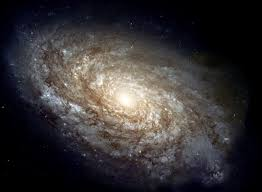
\includegraphics[width=0.5\textwidth]{galaxia.jpg}
    
    \note{La imagen muestra el \textit{render} de una galaxia, generada con 
    base en la información recabada por un telescopio de espacio profundo. 
    Esta imagen fue obtenida de \cite{hoover2010bio}.}
    \label{fig:galaxia}
    
\end{figure}
\end{verbatim}

Esto generará la siguiente figura:
\begin{figure}[h] 
    \centering\captionsetup{width=0.8\linewidth}
    \caption{Una imagen de una galaxia}
    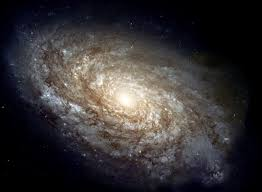
\includegraphics[width=0.5\textwidth]{galaxia.jpg}
    \note{La imagen muestra el \textit{render} de una galaxia, generada con  base en la información recabada por un telescopio de espacio profundo. Esta imagen fue obtenida de \cite{hoover2010bio}.}
    \label{fig:galaxia}   
\end{figure}

\newpage
A detalle
\begin{itemize}
    \itemsep 0em

    \item Las etiquetas \verb|\begin{figure} ... \end{figure}| indican el inicio y final de la figura, estas son parte de la sintaxis estándar de \LaTeX.

    \item La especificación \verb|[h]| dentro de corchetes en \verb|\begin{figure}[h]| indica en dónde deberá colocarse la figura. \verb|[t]| la coloca en la cima de la página, \verb|[b]| en el fondo y \verb|[h]| exactamente en el lugar donde aparece en el texto (esto es lo más similar a la manera en que añaden imágenes en Word). Es importante tomar en consideración que esta especificación es sólo una \textbf{sugerencia} para \LaTeX, ya que este colocará la imagen en donde quede mejor con respecto al espacio disponible. Si quiere forzar a \LaTeX a que respete la especificación, puede añadirle un signo de exclamación al final. Por ejemplo: \verb|\begin{figure}[h!]|.

    \item La etiqueta \verb|\centering| centra la figura y \verb|\captionsetup{width=0.8\linewidth}| indica que el título y la descripción ocuparán sólo el 80\% de los márgenes definidos para el texto. Estas etiquetas corresponden a estándares de formato para la plantilla y \textbf{siempre deberán incluirse tal cual y NO modificarse}.

    \item La etiqueta \verb|\caption{Título}| especifica el título de la figura. Este aparecerá por encima de la misma y alineado hacia la izquierda, y es el que también se ingresará automáticamente al listado. El título debe ser conciso; la descripción más profunda o detalles adicionales deberán colocarse en la Nota, al igual que la referencia bibliográfica si la hubiese. 

    \item \verb|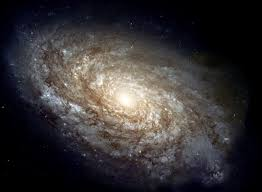
\includegraphics[width=0.5\textwidth]{galaxia.jpg}| hace referencia al archivo como tal de la figura y al tamaño deseado para la misma. En este caso, se está haciendo referencia al archivo de imagen \verb|galaxia.jpg| situado dentro de la carpeta \verb|figuras| en el árbol de navegación. Siempre que las figuras se encuentren dentro de esta carpeta se les podrá referenciar directamente por nombre y extensión de archivo. Con respecto al tamaño, puede establecerse tanto el alto como la altura directamente en unidades (el listado de unidades de tamaño que emplea \LaTeX puede consultarse en la documentación: \href{https://es.overleaf.com/learn/latex/Lengths_in_LaTeX}{https://es.overleaf.com/learn/latex/Lengths\_in\_LaTeX}). En este ejemplo, se está estableciendo el ancho, \verb|width|, como un porcentaje (de 0.0 a 1.0) del tamaño de los márgenes del texto (representado por la etiqueta \verb|\textwidth|). Para una referencia de cómo manejar el tamaño de figuras puede consultar la documentación: \href{https://www.overleaf.com/learn/latex/Questions/How_do_I_specify_the_size_of_an_image_in_LaTeX%3F}{https://www.overleaf.com/learn/latex/Questions/How\_do\_I\_specify\_the\_size\_of\_an\_image\_in\_LaTeX\%3F}.

    \item En caso de requerir una descripción adicional al título o bien brindar más detalles sobre la figura --pero que no se quiera que aparezcan en el índice de figuras--, debe emplearse la etiqueta \verb|\note{...}|. Dentro de esta etiqueta también deberá colocarse la referencia bibliográfica de la figura, si esta se obtuvo de esa manera. En caso que la figura sea de autoría propia deberá colocarse \verb|Elaboración propia.|.

    \item Finalmente, \verb|\label{...}| se emplea para crear una etiqueta que permita a \LaTeX encontrar el recurso cuando se utilicen referencias cruzadas. Todo recurso que quiera referenciarse dentro del texto debe contener una etiqueta y se recomienda emplear alguna convención de nombres para evitar el desorden. Por ejemplo, emplear \verb|\label{fig:nombre_figura}| para figuras, \verb|\label{tab:nombre_cuadro}| para cuadros y \verb|\label{eq:nombre_ecuación}| para ecuaciones. Para referenciar a la figura (o cuadro) dentro del texto se emplea el comando \verb|\ref{etiqueta}|. Por ejemplo, en la Figura \ref{fig:galaxia} puede verse el \textbf{render} de una galaxia, etc. Para el caso de ecuaciones se emplea pero \verb|\eqref{etiqueta}|.

\end{itemize}

Lo anterior se mantiene de la misma manera para cuadros, con la diferencia que deben emplearse las etiquetas \verb|\begin{table} ... \end{table}| para crearlos y deben ``programarse'' acorde a la sintaxis de \LaTeX. La recomendación es no hacer esto manualmente sino más bien emplear alguna herramienta como: 
\begin{itemize}
    \itemsep 0em
    \item \href{https://www.tablesgenerator.com/}{https://www.tablesgenerator.com/}
    \item \href{https://www.latex-tables.com/}{https://www.latex-tables.com/}
    \item \href{https://tableconvert.com/latex-generator}{https://tableconvert.com/latex-generator}
    \item \href{https://www.underleaf.ai/tools/latex-table-generator}{https://www.underleaf.ai/tools/latex-table-generator}
\end{itemize}

Por ejemplo, el Cuadro \ref{tab:experimentos_preliminares}
\begin{table}[h!]
    \centering\captionsetup{width=0.8\linewidth}
    \caption{Resultados del primer set de experimentos.}
    \begin{tabular}{c|ccc}
    \textbf{experimento} & variable 1 & variable 2 & variable 3 \\ \hline
    \textbf{1}           & 12.1       & 1          & 0          \\
    \textbf{2}           & -5.4       & 0          & 25         \\
    \textbf{3}           & 20.2       & 1          & 99        
    \end{tabular}
    \note{Los valores para la variable 2 son binarios mientras que los de la variable 3 son porcentuales. Elaboración propia.} 
    \label{tab:experimentos_preliminares}  
\end{table}

fue creado empleando el siguiente código:
\begin{verbatim}
\begin{table}[h]

    \centering\captionsetup{width=0.8\linewidth}
    \caption{Resultados del primer set de experimentos.}
    
    \begin{tabular}{c|ccc}
    \textbf{experimento} & variable 1 & variable 2 & variable 3 \\ \hline
    \textbf{1}           & 12.1       & 1          & 0          \\
    \textbf{2}           & -5.4       & 0          & 25         \\
    \textbf{3}           & 20.2       & 1          & 99        
    \end{tabular}
    
    \note{Los valores para la variable 2 son binarios mientras que los de 
    la variable 3 son porcentuales. Elaboración propia.}
    \label{tab:experimentos_preliminares}
    
\end{table}
\end{verbatim}

Para ecuaciones deben emplearse las etiquetas \verb|\begin{equation} ... \end{equation}| para crearlas. Dentro de estas la definición de las expresiones se hace mediante el modo matemático de \LaTeX. Si usted tiene experiencia previa con el mismo entonces puede escribir manualmente el código, sino también puede apoyarse de las siguientes herramientas:

\begin{itemize}
    \itemsep 0em

    \item \href{https://latexeditor.lagrida.com/}{https://latexeditor.lagrida.com/}

    \item \href{https://editor.codecogs.com/}{https://editor.codecogs.com/}

    \item \href{https://www.sciweavers.org/free-online-latex-equation-editor}{https://www.sciweavers.org/free-online-latex-equation-editor}

    \item \href{https://www.hostmath.com/}{https://www.hostmath.com/}

    \item En Overleaf puede trabajarse con un editor visual en lugar que el editor de código por defecto. Este editor permite crear ecuaciones de manera similar a Word. Puede ver cómo emplear este tipo de edición en el siguiente video: \href{https://youtu.be/hQ_sC0O-7Wg?si=r5gaTdL6e1LNkXML}{https://youtu.be/hQ\_sC0O-7Wg?si=r5gaTdL6e1LNkXML}.
\end{itemize}

o bien acudir a la documentación: \href{https://es.overleaf.com/learn/latex/Mathematical_expressions}{https://es.overleaf.com/learn/latex/Mathematical\_expressions}. Por ejemplo, la ecuación \eqref{eq:ejemplo_integral}
\begin{equation}
    F(x)=\int_{-\infty}^{x} f(s) ds,
    \label{eq:ejemplo_integral}
\end{equation}

puede generarse mediante el código:
\begin{verbatim}
\begin{equation}
    F(x)=\int_{-\infty}^{x} f(s) ds,
    \label{eq:ejemplo_integral}
\end{equation} 
\end{verbatim}


\section{Numeración y viñetas}

Para crear listados numerados o de viñetas, deben emplearse las etiquetas \newline \verb|\begin{enumerate} ... \end{enumerate}| o \verb|\begin{itemize} ... \end{itemize}| respectivamente. Cada ítem en el listado debe iniciarse con \verb|\item| y puede modularse la separación entre las mismas mediante \verb|\itemsep|. Por ejemplo, el siguiente código:
\begin{verbatim}
\begin{itemize}
    \item Primer elemento.

    \item Segundo elemento.

    \item Tercer elemento.

    \item Etc.
\end{itemize}
\end{verbatim}

produce el listado con viñetas:
\begin{itemize}
    \item Primer elemento.

    \item Segundo elemento.

    \item Tercer elemento.

    \item Etc.
\end{itemize}

Como segundo ejemplo, el código:
\begin{verbatim}
\begin{enumerate}
    \itemsep 0cm 
    
    \item Primer paso.

    \item Segundo paso.

    \item Tercer paso.

    \item Y así sucesivamente.
\end{enumerate}
\end{verbatim}

produce el listado numerado siguiente, en donde se empleó \verb|\itemsep| para eliminar el espacio entre elementos.
\begin{enumerate}
    \itemsep 0cm 
    
    \item Primer paso.

    \item Segundo paso.

    \item Tercer paso.

    \item Y así sucesivamente.
\end{enumerate}

\section{Referencias bibliográficas}

El manejo de referencias bibliográficas dentro de la plantilla se trabaja mediante BibTeX (\href{https://www.overleaf.com/learn/latex/Bibliography_management_with_bibtex}{https://www.overleaf.com/learn/latex/Bibliography\_management\_with\_bibtex}). Este permite crear referencias cruzadas simples a las referencias mediante el comando \verb|\cite{referencia}|, siempre y cuando la referencia se haya definido correctamente dentro del fichero \verb|m-bibliografia.bib|. Si bien puede crearse manualmente cada ficha bibliográfica, como se muestra en el siguiente ejemplo (que aparece dentro del fichero \verb|m-bibliografia.bib|) 

\begin{verbatim}
@article{park2014design,
  title={Design and control of a bio-inspired soft wearable robotic device for 
  ankle--foot rehabilitation},
  author={Park, Yong-Lae and Chen, Bor-rong and P{\'e}rez-Arancibia, N{\'e}stor 
  O and Young, Diana and Stirling, Leia and Wood, Robert J and Goldfield, Eugene 
  C and Nagpal, Radhika},
  journal={Bioinspiration \& biomimetics},
  volume={9},
  number={1},
  pages={016007},
  year={2014},
  publisher={IOP Publishing}
}
\end{verbatim}

se prefiere emplear herramientas que automaticen este proceso, ya que no sólo las fichas individuales son extensas sino que cambian de campos requeridos dependiendo del tipo de fuente. Dos de las herramientas de manejo de referencias estándar en investigación son Mendeley (\href{https://www.mendeley.com/search/}{https://www.mendeley.com/search/}) y Zotero (\href{https://www.zotero.org/}{https://www.zotero.org/}), con las cuales puede generarse el contenido del fichero \texttt{.bib} automáticamente, como se muestra en el siguiente video \href{https://youtu.be/avwPBvaYgw4?si=YBZj3l3QhzO47oDS}{https://youtu.be/avwPBvaYgw4?si=YBZj3l3QhzO47oDS}.
 
\ifdefined\usarAPA
    Para la referencia que se definió anteriormente, basta con emplear \verb|\parencite{park2014design}| para que aparezca dentro del texto de la siguiente manera \parencite{park2014design}.
\else
    Para la referencia que se definió anteriormente, basta con emplear \verb|\cite{park2014design}| para que aparezca dentro del texto de la siguiente manera \cite{park2014design}.
\fi

En caso no tenga experiencia previa empleando Mendeley y/o Zotero, puede consultar los recursos dentro de la guía para la redacción de trabajos de graduación.

\section{Personalización}

La plantilla permite cierto grado de personalización, accesible principalmente a través del resto del archivo \verb|0-datos_estudiante.tex|. Primero, puede emplearse el símbolo \verb|%| para activar y desactivar capítulos, secciones y configuraciones adicionales. Por ejemplo, en caso de querer omitir el capítulo de Prefacio basta con preceder su línea respectiva con el símbolo \verb|%|, es decir, \verb|%\def \CAPprefacio {Prefacio}|. Expandiendo esta funcionalidad, la siguiente configuración

\begin{verbatim}
% Capítulos pre-definidos
% -------------------------------------------------------------------------
% Comentar las líneas de las secciones que desean omitirse, por defecto se 
% se incluyen todas.
\def \CAPprefacio {Prefacio}
\def \CAPantecedentes {Antecedentes}
%\def \CAPanexos {Anexos}
\def \CAPglosario {Glosario}

% Sólo puede activarse UNA de las siguientes tres opciones, dependiendo de 
lo que se requiera (revisar la guía de redacción de trabajos de graduación).
\def \CAPhipotesis {Hipótesis}
%\def \CAPdefinicion {Definición del problema}
%\def \CAPalcance {Alcance}
\end{verbatim}

hace que el trabajo incluya los capítulos de Prefacio, Antecedentes y Glosario pero no el de Anexos. Adicionalmente, entre las tres opciones a emplear para el capítulo de Hipótesis / Definición del problema / Alcance, se selecciona la de Hipótesis.

Puede emplearse un estilo de referencias APA, en lugar del estándar IEEE, activando el atributo \verb|\usarAPA|:
\begin{verbatim}
% Referencias: Puede des-comentar la siguiente línea para utilizar el formato de 
referencias APA
%\def \usarAPA {Usar formato APA}
\end{verbatim}

También puede configurarse para que la plantilla genere la hoja de firmas empleando la información del asesor y los evaluadores --para luego ser firmada en el documento como tal-- o bien que utilice una hoja de firmas definida en un archivo \texttt{.pdf} externo. En caso de emplear la segunda opción debe reemplazarse el archivo \verb|hoja_firmas.pdf| con la hoja de firmas y desactivar el atributo \verb|\GENfirmas|, es decir, la línea correspondiente debe verse como \verb|%\def \GENfirmas {Hoja de firmas}|.

Finalmente, la plantilla permite modificar la imagen en la portada mediante el atributo \verb|\imagenportada|:
\begin{verbatim}
% Portada: Puede cambiarse la imagen en la portada al cambiar el nombre del 
% archivo siguiente. NOTA: la imagen debe tener la suficiente resolución 
(1920x768, o más grande pero con una relación 2.5:1) para cubrir el área 
designada. Por defecto se coloca la imagen del CIT.
\def \imagenportada {plantilla/portadacit-real.png}
\end{verbatim}
Para hacerlo, basta con reemplazar la referencia a la imagen por defecto por la que quiera emplearse (si la coloca dentro de la carpeta de \verb|figuras| sólo deberá colocar el nombre del archivo, sin la referencia a la carpeta). Tome nota que la imagen deberá tener una resolución mínima de \texttt{1920 x 768}, o bien una resolución más grande pero que mantenga una relación de aspecto de \texttt{2.5:1}.

\subsection{Capítulos}

Por la variabilidad que existe entre los trabajos de graduación dependiendo de la modalidad de graduación, carrera y facultad, la plantilla no establece capítulos predeterminados más allá de los obligatorios para todos los casos. Por lo tanto, es responsabilidad del usuario definir los capítulos que necesite dentro del archivo \verb|j-capitulos.tex|. Estos se añadirán automáticamente al índice general junto con las secciones del siguiente nivel de indentación. 

Para definir capítulos adicionales se emplea el comando \verb|\chapter{Nombre del capítulo}|. Pueden definirse --dentro de cualquier capítulo del trabajo-- secciones, sub-secciones y hasta sub sub-secciones, empleando los comandos \verb|\section{...}|, \verb|\subsection{...}| y \\ \verb|\subsubsection{...}| respectivamente. El siguiente código entonces
\begin{verbatim}
\chapter{Ejemplo de capítulo}

\section{Ejemplo de sección}

\subsection{Ejemplo de sub-sección}

\subsubsection{Ejemplo de sub sub-sección}
\end{verbatim}

define un capítulo nuevo con algunas secciones y sub-secciones de prueba

\subsection{Glosario}

El glosario es un capítulo opcional. Se compone de una lista de palabras relacionadas en la investigación, pero desconocidas para el lector. Estas deben presentarse en orden alfabético, junto con su definición. 

Siempre y cuando se encuentre activado, el archivo  \verb|o-glosario.tex| puede emplearse para definir el glosario acorde a la sintaxis de \LaTeX: \href{https://es.overleaf.com/learn/latex/Glossaries}{https://es.overleaf.com/learn/latex/Glossaries}. De esta manera es posible automatizar la generación del glosario y se permitirá el uso de referencias cruzadas para los términos dentro del mismo. 

Por ejemplo, dentro del archivo \verb|o-glosario.tex| se encuentra la definición del término \gls{latex} como
\begin{verbatim}
\newglossaryentry{latex}
{
    name=latex,
    description={Es un lenguaje de marcado adecuado especialmente para la 
    creación de documentos científicos}
}    
\end{verbatim}

Luego de estar definido el término puede emplearse dentro del texto mediante \verb|\gls{latex}|, o bien \verb|\Gls{latex}| si quiere emplearse con mayúscula. Al hacer esto los términos definidos dentro del glosario deberían aparecer de la siguiente forma, por ejemplo, dentro del texto: \gls{formula}, \Gls{latex}.


\chapter{Ejemplo de capítulo}

\section{Ejemplo de sección}
\subsection{Ejemplo de sub-sección}

\subsubsection{Ejemplo de sub sub-sección}
